\begin{figure}[t!]
  \centering
  \subfloat[Current state-of-practice]{%
    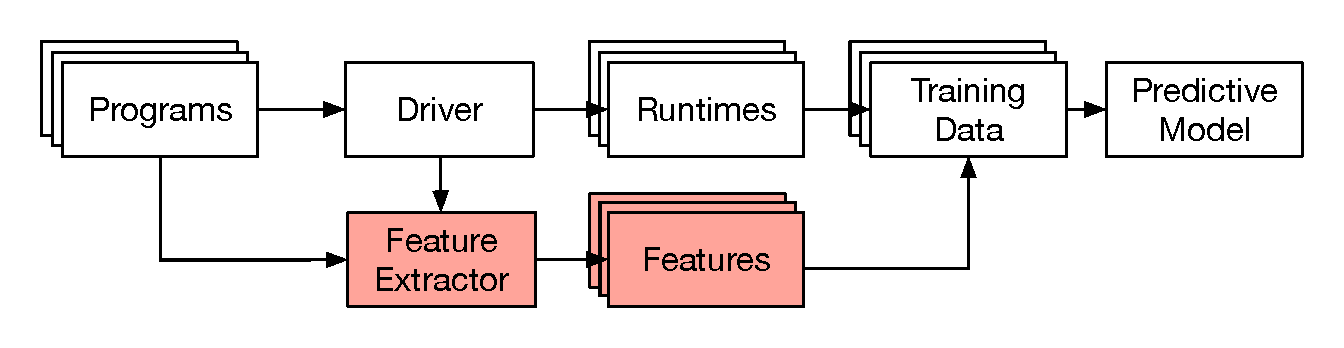
\includegraphics[width=.95\columnwidth]{img/training_model_a}%
    \label{fig:overview-a}%
  }\\*%
  \subfloat[Our proposal]{%
    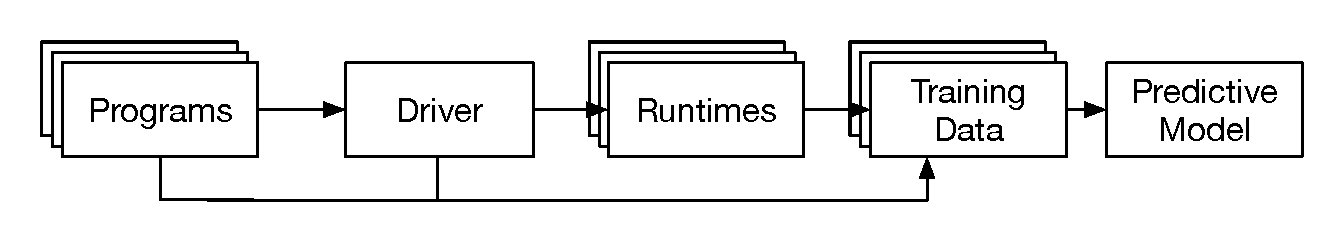
\includegraphics[width=.95\columnwidth]{img/training_model_b}%
    \label{fig:overview-b}%
  }%
  \vspace{-.4em}%
  \caption{%
    Building a predictive model. The model is originally trained on performance
    data and features extracted from the source code and the runtime behavior.
    We propose bypassing feature extraction, instead learning directly over raw
    program source code.%
  }%
  \label{fig:overview}
\end{figure}
